%% abtex2-modelo-trabalho-academico.tex, v-1.9.5 laurocesar
%% Copyright 2012-2015 by abnTeX2 group at http://www.abntex.net.br/
%%
%% This work may be distributed and/or modified under the
%% conditions of the LaTeX Project Public License, either version 1.3
%% of this license or (at your option) any later version.
%% The latest version of this license is in
%%   http://www.latex-project.org/lppl.txt
%% and version 1.3 or later is part of all distributions of LaTeX
%% version 2005/12/01 or later.
%%
%% This work has the LPPL maintenance status `maintained'.
%%
%% The Current Maintainer of this work is the abnTeX2 team, led
%% by Lauro César Araujo. Further information are available on
%% http://www.abntex.net.br/
%%
%% This work consists of the files abntex2-modelo-trabalho-academico.tex,
%% abntex2-modelo-include-comandos and abntex2-modelo-references.bib
%%

% ------------------------------------------------------------------------
% ------------------------------------------------------------------------
% abnTeX2: Modelo de Trabalho Academico (tese de doutorado, dissertacao de
% mestrado e trabalhos monograficos em geral) em conformidade com
% ABNT NBR 14724:2011: Informacao e documentacao - Trabalhos academicos -
% Apresentacao
% ------------------------------------------------------------------------
% ------------------------------------------------------------------------

\documentclass[
	% -- opções da classe memoir --
	12pt,				% tamanho da fonte
	%openright,			% capítulos começam em pág ímpar (insere página vazia caso preciso)
	%openany, % a chapter can start on any page, then many classes support option openany, e.g.:
	oneside, %% straight PAGE alignment 
 % With twoside layout (default for class book) chapters start at odd numbered pages and sometimes LaTeX needs to insert a page to ensure this.
	%twoside,			% para impressão em verso e anverso. Oposto a oneside
	a4paper,			% tamanho do papel.
	% -- opções da classe abntex2 --
	%chapter=TITLE,		% títulos de capítulos convertidos em letras maiúsculas
	%section=TITLE,		% títulos de seções convertidos em letras maiúsculas
	%subsection=TITLE,	% títulos de subseções convertidos em letras maiúsculas
	%subsubsection=TITLE,% títulos de subsubseções convertidos em letras maiúsculas
	% -- opções do pacote babel --
	english,			% idioma adicional para hifenização
	french,				% idioma adicional para hifenização
	spanish,			% idioma adicional para hifenização
	brazil				% o último idioma é o principal do documento
	]{abntex2}

% ---
% Pacotes básicos
% ---
\usepackage{lmodern} % para fontes Latin Modern
\usepackage[T1]{fontenc}		% Selecao de codigos de fonte.
\usepackage[utf8]{inputenc}		% Codificacao do documento (conversão automática dos acentos)
\usepackage{lastpage}			% Usado pela Ficha catalográfica
\usepackage{indentfirst}		% Indenta o primeiro parágrafo de cada seção.
\usepackage{color}				% Controle das cores
\usepackage{graphicx}			% Inclusão de gráficos
\usepackage{microtype} 			% para melhorias de justificação
\usepackage{booktabs}
\usepackage{graphicx}
\usepackage[table,xcdraw]{xcolor}
\usepackage{float}
\usepackage{listings}
\usepackage{ragged2e}
\usepackage{tabto}

\usepackage{subfig} % double image add to page % below
\usepackage{caption}
\usepackage{subcaption}
\usepackage{amsmath} % math matrix
% --- https://www.overleaf.com/learn/latex/Code_listing
\usepackage{amssymb} % \triangleq
\usepackage{comment}
%\usepackage{setspace}
%\usepackage{empheq} %in case of error delete it 

% label to verbatim
% https://tex.stackexchange.com/questions/345926/crossreferencing-verbatim
%\BeforeBeginEnvironment{verbatim}{%
%\refstepcounter{myverb}%
%\noindent\textbf{Verbatim stuff \themyverb}%
%}

%\usepackage{caption}
%\usepackage{subcaption}
\usepackage{float}


%Solution 3: Suppress chapter number in section numbering If you must keep the class with chapters but don’t want them to appear in section numbering: Add this to the preamble:
\renewcommand{\thesection}{\arabic{section}}



\usepackage{array,tabularx,calc}  %https://tex.stackexchange.com/questions/95838/how-to-write-a-perfect-equation-parameters-description


\newlength{\conditionwd}
\newenvironment{conditions}[1][Onde:]
  {%
   #1\tabularx{\textwidth-\widthof{#1}}[t]{
     >{$}l<{$} @{${}={}$} X@{}
   }%
  }
  {\endtabularx\\[\belowdisplayskip]}



\usepackage{xcolor}
\renewcommand\lstlistingname{Lista de código}
\renewcommand\lstlistlistingname{Lista de trechos de código}

% https://tex.stackexchange.com/questions/111580/removing-an-unwanted-page-between-two-chapters
\let\cleardoublepage\clearpage % Unwanted one-page gap between two chapters can be eliminated using the syntax




\definecolor{codegreen}{rgb}{0,0.6,0}
\definecolor{codegray}{rgb}{0.5,0.5,0.5}
\definecolor{codepurple}{rgb}{0.58,0,0.82}
\definecolor{backcolour}{rgb}{0.95,0.95,0.92}
%ref TROUBLESHOOTING = https://tex.stackexchange.com/questions/24528/having-problems-with-listings-and-utf-8-can-it-be-fixed
%ref = https://www.overleaf.com/learn/latex/Code_listing
\lstdefinestyle{mystyle}{
    backgroundcolor=\color{backcolour},
    commentstyle=\color{codegreen},
    keywordstyle=\color{magenta},
    numberstyle=\tiny\color{codegray},
    stringstyle=\color{codepurple},
    basicstyle=\ttfamily\footnotesize,
    breakatwhitespace=false,
    breaklines=true,
    captionpos=b,
    keepspaces=true,
    numbers=left,
    numbersep=5pt,
    showspaces=false,
    showstringspaces=false,
    showtabs=false,
    tabsize=2,
    inputencoding = utf8,  % Input encoding
    extendedchars = true,  % Extended ASCII
    literate      =        % Support additional characters
      {á}{{\'a}}1  {é}{{\'e}}1  {í}{{\'i}}1 {ó}{{\'o}}1  {ú}{{\'u}}1
      {Á}{{\'A}}1  {É}{{\'E}}1  {Í}{{\'I}}1 {Ó}{{\'O}}1  {Ú}{{\'U}}1
      {à}{{\`a}}1  {è}{{\`e}}1  {ì}{{\`i}}1 {ò}{{\`o}}1  {ù}{{\`u}}1
      {À}{{\`A}}1  {È}{{\`E}}1  {Ì}{{\`I}}1 {Ò}{{\`O}}1  {Ù}{{\`U}}1
      {ä}{{\"a}}1  {ë}{{\"e}}1  {ï}{{\"i}}1 {ö}{{\"o}}1  {ü}{{\"u}}1
      {Ä}{{\"A}}1  {Ë}{{\"E}}1  {Ï}{{\"I}}1 {Ö}{{\"O}}1  {Ü}{{\"U}}1
      {â}{{\^a}}1  {ê}{{\^e}}1  {î}{{\^i}}1 {ô}{{\^o}}1  {û}{{\^u}}1
      {Â}{{\^A}}1  {Ê}{{\^E}}1  {Î}{{\^I}}1 {Ô}{{\^O}}1  {Û}{{\^U}}1
      {œ}{{\oe}}1  {Œ}{{\OE}}1  {æ}{{\ae}}1 {Æ}{{\AE}}1  {ß}{{\ss}}1
      {ẞ}{{\SS}}1  {ç}{{\c{c}}}1 {Ç}{{\c{C}}}1 {ø}{{\o}}1  {Ø}{{\O}}1
      {å}{{\aa}}1  {Å}{{\AA}}1  {ã}{{\~a}}1  {õ}{{\~o}}1 {Ã}{{\~A}}1
      {Õ}{{\~O}}1  {ñ}{{\~n}}1  {Ñ}{{\~N}}1  {¿}{{?`}}1  {¡}{{!`}}1
      {°}{{\textdegree}}1 {º}{{\textordmasculine}}1 {ª}{{\textordfeminine}}1
      {£}{{\pounds}}1  {©}{{\copyright}}1  {®}{{\textregistered}}1
      {«}{{\guillemotleft}}1  {»}{{\guillemotright}}1  {Ð}{{\DH}}1  {ð}{{\dh}}1
      {Ý}{{\'Y}}1    {ý}{{\'y}}1    {Þ}{{\TH}}1    {þ}{{\th}}1    {Ă}{{\u{A}}}1
      {ă}{{\u{a}}}1  {Ą}{{\k{A}}}1  {ą}{{\k{a}}}1  {Ć}{{\'C}}1    {ć}{{\'c}}1
      {Č}{{\v{C}}}1  {č}{{\v{c}}}1  {Ď}{{\v{D}}}1  {ď}{{\v{d}}}1  {Đ}{{\DJ}}1
      {đ}{{\dj}}1    {Ė}{{\.{E}}}1  {ė}{{\.{e}}}1  {Ę}{{\k{E}}}1  {ę}{{\k{e}}}1
      {Ě}{{\v{E}}}1  {ě}{{\v{e}}}1  {Ğ}{{\u{G}}}1  {ğ}{{\u{g}}}1  {Ĩ}{{\~I}}1
      {ĩ}{{\~\i}}1   {Į}{{\k{I}}}1  {į}{{\k{i}}}1  {İ}{{\.{I}}}1  {ı}{{\i}}1
      {Ĺ}{{\'L}}1    {ĺ}{{\'l}}1    {Ľ}{{\v{L}}}1  {ľ}{{\v{l}}}1  {Ł}{{\L{}}}1
      {ł}{{\l{}}}1   {Ń}{{\'N}}1    {ń}{{\'n}}1    {Ň}{{\v{N}}}1  {ň}{{\v{n}}}1
      {Ő}{{\H{O}}}1  {ő}{{\H{o}}}1  {Ŕ}{{\'{R}}}1  {ŕ}{{\'{r}}}1  {Ř}{{\v{R}}}1
      {ř}{{\v{r}}}1  {Ś}{{\'S}}1    {ś}{{\'s}}1    {Ş}{{\c{S}}}1  {ş}{{\c{s}}}1
      {Š}{{\v{S}}}1  {š}{{\v{s}}}1  {Ť}{{\v{T}}}1  {ť}{{\v{t}}}1  {Ũ}{{\~U}}1
      {ũ}{{\~u}}1    {Ū}{{\={U}}}1  {ū}{{\={u}}}1  {Ů}{{\r{U}}}1  {ů}{{\r{u}}}1
      {Ű}{{\H{U}}}1  {ű}{{\H{u}}}1  {Ų}{{\k{U}}}1  {ų}{{\k{u}}}1  {Ź}{{\'Z}}1
      {ź}{{\'z}}1    {Ż}{{\.Z}}1    {ż}{{\.z}}1    {Ž}{{\v{Z}}}1
      % ¿ and ¡ are not correctly displayed if inconsolata font is used
      % together with the lstlisting environment. Consider typing code in
      % external files and using \lstinputlisting to display them instead.      
}

\lstset{style=mystyle}



% ------------------------------------------------------------------------
% ------------------------------------------------------------------------
%The error indicates that the \uppercase command is being used in a context where it is not allowed, specifically within a PDF string. However, no direct usage of %\uppercase was found in the main.tex file. It might be used indirectly or through another command.
%To resolve this, I will add the \pdfstringdefDisableCommands command in the %preamble to handle \uppercase properly.
\pdfstringdefDisableCommands{\let\uppercase\relax}
% ------------------------------------------------------------------------
% ------------------------------------------------------------------------
% Pacotes adicionais, usados apenas no âmbito do Modelo Canônico do abnteX2
% ---
\usepackage{lipsum}				% para geração de dummy text
% ---
\usepackage{tikz}

% ---
% Pacotes de citações
% ---
%\usepackage[backref=true, colorlinks=true, linkcolor=blue, citecolor=blue, urlcolor=blue]{hyperref}
\usepackage[unicode,brazilian,hyperpageref]{backref}
%\usepackage[brazilian,hyperpageref]{backref}	 % Paginas com as citações na bibl

%%%%%%--- test pacote USPSC ---%%%%%%%%%
%%%%%%--- test pacote USPSC ---%%%%%%%%%
%%%%%%--- test pacote USPSC ---%%%%%%%%%
\usepackage[alf, abnt-emphasize=bf, abnt-thesis-year=both, abnt-repeated-author-omit=no, abnt-last-names=abnt, abnt-etal-cite=3, abnt-etal-list=3, abnt-etal-text=it, abnt-and-type=e, abnt-doi=doi, abnt-url-package=none, abnt-verbatim-entry=no]{abntex2cite}
\bibliographystyle{USPSC-classe/abntex2-alf-USPSC}

% ----
% Compatibilização com a ABNT NBR 6023:2018 e 10520:2023
% Para tirar <> da URL e tornar as expressões latinas em itálico
\usepackage{USPSC-classe/ABNT6023-10520}
% As demais compatibilizações estão nos arquivos abntex2-alf-USPSC.bst,abntex2-alfeng-USPSC.bst, abntex2-num-USPSC.bst e abntex2-numeng-USPSC.bst, dependendo do idioma do textos e se o sistemas de chamada for autor-data ou numérico, conforme explicitado acima.
% ----

%%%%%%--- test pacote USPSC ---%%%%%%%%%
%%%%%%--- test pacote USPSC ---%%%%%%%%%
%%%%%%--- test pacote USPSC ---%%%%%%%%%

%\usepackage[brazilian,hyperpageref]{backref}

%%%% WORLING REF BELOW - UNCOMMENT  %%%%
%\usepackage[alf]{abntex2cite}	% Citações padrão ABNT

% --- checkmark
\usepackage{tikz}
\def\checkmark{\tikz\fill[scale=0.4](0,.35) -- (.25,0) -- (1,.7) -- (.25,.15) -- cycle;} 


% First pip install pygments

% CONFIGURAÇÕES DE PACOTES
% ---

% ---https://mirrors.ibiblio.org/CTAN/macros/latex/contrib/abntex2/doc/abntex2cite-alf.pdf
% Configurações do pacote backref
% Usado sem a opção hyperpageref de backref

%\begin{comment}

%\usepackage[backref=true, colorlinks=true, linkcolor=blue, citecolor=blue, urlcolor=blue]{hyperref}

% Personalizações devem vir depois de carregar o pacote
\renewcommand{\backrefpagesname}{Citado na(s) página(s):~}
\renewcommand{\backref}{}
\renewcommand*{\backrefalt}[4]{
  \ifcase #1
    Nenhuma citação no texto.%
  \or
    Citado na página #2.%
  \else
    Citado nas páginas #2.%
  \fi
}

%\end{comment}
% --- https://mirrors.ibiblio.org/CTAN/macros/latex/contrib/abntex2/doc/abntex2cite-alf.pdf

% ---
% Informações de dados para CAPA e FOLHA DE ROSTO
% ---
%\local{Campos dos Goytacazes, RJ}
%\data{\today}
%\orientador{Prof. Dr. Annabell Del Real Tamariz}
%\coorientador{Equipe \abnTeX}

% O preambulo deve conter o tipo do trabalho, o objetivo,
% o nome da instituição e a área de concentração
%\preambulo{Trabalho de Conclusão de Curso apresentado ao Curso de Graduação em Ciência da Computação da Universidade Estadual do Norte Fluminense Darcy Ribeiro como requisito para a obtenção do título de Bacharel em Ciência da Computação, sob orientação de Annabell Del Real Tamariz}
% ---

% ---
% Configurações de aparência do PDF final

% alterando o aspecto da cor azul
\definecolor{blue}{RGB}{41,5,195}

% informações do PDF
\makeatletter
\hypersetup{
     	%pagebackref=true,
		pdftitle={\@title},
		pdfauthor={\@author},
    	pdfsubject={\imprimirpreambulo},
	    pdfcreator={LaTeX with abnTeX2},
		pdfkeywords={abnt}{latex}{abntex}{abntex2}{trabalho acadêmico},
		colorlinks=true,       		% false: boxed links; true: colored links
    	linkcolor=blue,          	% color of internal links
    	citecolor=blue,        		% color of links to bibliography
    	filecolor=magenta,      		% color of file links
		urlcolor=blue,
		bookmarksdepth=4
}
\makeatother
% ---
% ---
% Seguindo a NBR 6023 joao
% Seguindo a NBR 6023 https://github.com/abntex/abntex2/issues/210#issuecomment-633050367
\usepackage{url6023}
%\ProvidesPackage{url6023}


% Seguindo a NBR6023

% ---
% Espaçamentos entre linhas e parágrafos
% ---

% O tamanho do parágrafo é dado por:
\setlength{\parindent}{1.3cm}

% Controle do espaçamento entre um parágrafo e outro:
\setlength{\parskip}{0.2cm}  % tente também \onelineskip

% ---
% compila o indice
% ---
\makeindex
% ---

% ----
% Início do documento
% ----
\usepackage{titlesec}

% Redefine the section format according to ABNT 2
\titleformat{\section}[block]{\normalfont\bfseries\Large}{\thesection}{1em}{} % Main section
\titleformat{\subsection}[block]{\normalfont\bfseries\large}{\thesubsection}{1em}{} % Subsection
\titleformat{\subsubsection}[block]{\normalfont\normalsize}{\thesubsubsection}{1em}{} % Subsubsection

% Add space before and after sections, according to ABNT 2
\titlespacing*{\section}{0pt}{2ex plus .2ex minus .2ex}{1ex plus .2ex}  % Space before and after main section
\titlespacing*{\subsection}{0pt}{1.5ex plus .2ex minus .2ex}{1ex plus .2ex} % Space before and after subsection
\titlespacing*{\subsubsection}{0pt}{1.5ex plus .2ex minus .2ex}{1ex plus .2ex} % Space before and after subsubsection


%% citation
%\usepackage[style=abnt, language=brazil]{biblatex}
%\addbibresource{bibli.bib} % Substitua pelo nome do seu arquivo .bib

%% citation

\titulo{\textbf{Integração Dinâmica de Percepção, Planejamento e Controle para Navegação Autônoma no Simulador CARLA}}
\autor{Daniel Terra Gomes}
%\local{Campos dos Goytacazes, RJ}
\data{\today}
%\tipotrabalho{Projeto de Pesquisa}
\makeatletter
\def\maketitle{
    \begin{center}
        \LARGE \textbf{\thetitle} \\[1em]
        \large {\theauthor}\\ [0.5em]
        \small \thedate
    \end{center}
}
\makeatother


\begin{document}

\maketitle

\section{Introdução}

O avanço tecnológico no setor automotivo, especialmente em veículos elétricos e direção autônoma, vem transformando profundamente a mobilidade urbana \cite{sebo2024impact}. Empresas como ZOOX\textsuperscript{\textregistered} e WAYMO\textsuperscript{\textregistered} investem fortemente no desenvolvimento de tecnologias capazes de reduzir acidentes de trânsito, otimizar o fluxo viário e reformular a logística \cite{Center_of_Automotive_Management2022}. A redução de acidentes, atribuída majoritariamente a falhas humanas \cite{nhtsa_crash_causation}, é um dos benefícios mais promissores, destacando a importância da automação veicular para uma condução mais segura \cite{okpono2024advanced}.

Nesse cenário, a direção autônoma abrange quatro módulos principais: percepção, estimação de estado, planejamento de movimento e controle \cite{reinholtz2007darpa, paden2016survey}. A percepção visual, impulsionada pelo desenvolvimento de redes neurais profundas como o YOLO \cite{redmon2016lookonceunifiedrealtime, wang_yolov1_to_yolov10}, tem se destacado ao permitir detecção eficiente de objetos em tempo real, fator crucial para a navegação segura.

Durante a graduação, entre 2022 e 2025, foram realizadas três etapas de Iniciação Científica, culminando na implementação de um veículo autônomo funcional no simulador CARLA \cite{gomes2025relatorio, dosovitskiy2017carla}. Apesar dos avanços, a integração entre percepção e planejamento ainda ocorria de forma estática, limitando a capacidade reativa do sistema. Frente a isso, este trabalho tem como objetivo propor uma arquitetura dinâmica de navegação autônoma, com integração reativa entre percepção, planejamento e controle no simulador CARLA. A percepção baseada em YOLO detectará objetos em tempo real, alimentando uma Máquina de Estados Finitos e um \textit{Lattice Planner}, que coordenarão a tomada de decisão e o planejamento da trajetória, enviados aos controladores \textit{PID} e \textit{Pure Pursuit} \cite{University_of_Toronto2018-fe}.

Desse modo, a realização desta pesquisa se justifica pela importância de desenvolver sistemas de navegação autônoma mais adaptativos e reativos, capazes de operar de forma robusta em cenários dinâmicos e imprevisíveis, uma demanda crescente no contexto da mobilidade urbana inteligente e mais segura \cite{sebo2024impact}. Além disso, o uso do simulador CARLA oferece uma plataforma segura, acessível e realista para a experimentação e validação de soluções complexas, contribuindo para o avanço científico e tecnológico \cite{dosovitskiy2017carla}.



\section{Referencial Teórico}

O desenvolvimento de veículos autônomos (VA) exige a integração eficaz dos módulos de percepção, planejamento e controle para garantir a navegação segura em ambientes urbanos. Trabalhos como \citeonline{andrade_object_detection_distance} e \citeonline{sanchez_speed_sign_detection} exploraram a detecção de objetos e sinais de trânsito utilizando o algoritmo YOLO; entretanto, não avançaram para a construção de um sistema autônomo completo. Da mesma forma, \citeonline{Gao_2021} e \citeonline{ahammed2024computer} trataram da percepção visual, mas sem propor a integração com planejamento e controle.

Projetos de referência, como o desenvolvido no \textit{DARPA Urban Challenge} \cite{reinholtz2007darpa}, demonstraram a viabilidade da integração de módulos para a navegação autônoma em ambientes complexos. Nesse contexto, sistemas robustos foram implementados, consolidando a percepção, o planejamento de trajetórias e o controle dinâmico em um único arcabouço operacional.
Em ambientes simulados, o simulador Carla \cite{dosovitskiy2017carla} tem sido amplamente utilizado para validação de sistemas autônomos, permitindo a reprodução de cenários urbanos realistas com baixo custo e segurança. Estudos recentes, como \citeonline{kim2023challenges} e \citeonline{W4389342036}, empregaram o CARLA para testar algoritmos de percepção e planejamento, reforçando sua importância como plataforma de pesquisa.

Diferenciando-se dos trabalhos citados, esta pesquisa propõe a integração dos módulos de percepção, planejamento e controle no ambiente do CARLA, aproximando-se das práticas industriais observadas em sistemas de VA avançados \cite{University_of_Toronto2018-fe}. Esta abordagem busca contribuir para o desenvolvimento de VA mais completos e eficientes, avançando nos trabalhos discutido em \citeonline{gomes2025relatorio}.

\section{Metodologia}

A pesquisa será aplicada, de abordagem quantitativa e natureza experimental, com objetivo descritivo. O cenário de testes será o simulador CARLA, sendo as implementações e avaliações realizadas no computador do pesquisador e/ou no laboratório de simulação computacional da instituição.

O projeto adota uma arquitetura modular para VA em ambiente simulado, conforme a Figura~\ref{fig:arquiteturaa}, dividida em três camadas: percepção ambiental, planejamento de movimento e controle.
A camada de percepção usará a saída da câmera do CARLA para detectar e classificar objetos com algoritmos como redes YOLO. Em seguida, o planejamento de movimento será composto por uma Máquina de Estados Finitos e \textit{Lattice Planner}. A camada de controle executará os comandos de direção e velocidade utilizando controladores \textit{PID} e \textit{Pure Pursuit}.

O sistema contará ainda com um módulo de assistência ao condutor, fornecendo \textit{feedback} em tempo real. O desenvolvimento modular permitirá avaliações isoladas dos componentes, com testes controlados baseados em métricas como evasão de obstáculos, tempo de resposta e número de colisões evitadas. A análise dos dados será feita estatisticamente, validando a robustez da arquitetura em cenários dinâmicos.

\begin{figure}[H]
    \centering
    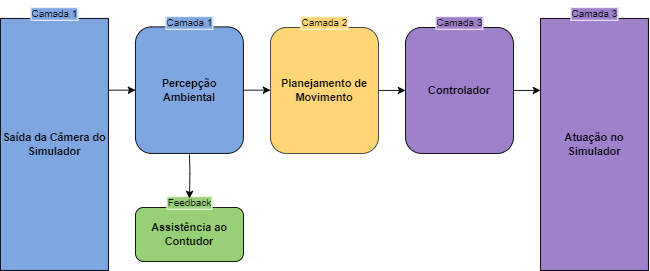
\includegraphics[width=0.6\textwidth]{Figures/ArquiteturadeSoftware.png}
    \caption{Arquitetura do Software.}
    \label{fig:arquiteturaa}
    \small\textbf{Fonte:} Elaborado pelo autor.
\end{figure}



%%%%----
%%%%----
\section{Cronograma}

O desenvolvimento deste projeto está previsto para ocorrer ao longo de quatro semestres letivos, com início em 2025.2. As atividades incluem aprofundamento teórico por meio de disciplinas, implementação incremental da proposta, testes e validações no simulador CARLA, além da redação da dissertação. O cronograma está organizado conforme apresentado na Tabela~\ref{tab:etapas}.

% Please add the following required packages to your document preamble:
% \usepackage{booktabs}
% \usepackage{graphicx}
% \usepackage[table,xcdraw]{xcolor}
% If you use beamer only pass "xcolor=table" option, i.e. \documentclass[xcolor=table]{beamer}
\begin{table}[H]
\centering
\resizebox{\textwidth}{!}{%
\begin{tabular}{@{}|lllllllllllll|@{}}

\cmidrule(l){1-13}

  \multicolumn{1}{|c}{} &
  \multicolumn{1}{c}{} &
  \multicolumn{1}{c}{\textbf{1º}} &
  \multicolumn{1}{c}{\textbf{ano}} &
  \multicolumn{1}{c}{} &
  \multicolumn{1}{c|}{} &
  \multicolumn{1}{c}{} &
  \multicolumn{1}{c}{} &
  \multicolumn{1}{c}{\textbf{2º}} &
  \multicolumn{1}{c}{\textbf{ano}} &
  \multicolumn{1}{c}{} &
  \multicolumn{1}{c}{} &
  \multicolumn{1}{c|}{}  \\

\cmidrule(l){1-13}


  \multicolumn{1}{|c}{} &
  \multicolumn{1}{c}{\textbf{2025.2}} &
  \multicolumn{1}{c|}{} &
    \multicolumn{1}{c}{} &

  \multicolumn{1}{c}{\textbf{2026.1}} &
  \multicolumn{1}{c|}{} &
    \multicolumn{1}{c}{} &

  \multicolumn{1}{c}{\textbf{2026.2}} &
  \multicolumn{1}{c|}{} &
    \multicolumn{1}{c}{} &

    \multicolumn{1}{c}{\textbf{2027.1}} &
        \multicolumn{1}{c}{} &
  \multicolumn{1}{c|}{} \\ \midrule

 
\multicolumn{1}{|l}{\cellcolor[HTML]{ebaca9}} 

\cellcolor[HTML]{ebaca9}&
   \cellcolor[HTML]{ebaca9} {\textbf{Levantamento}}&
  \cellcolor[HTML]{ebaca9} & {\textbf{\&}}
  \cellcolor[HTML]{ebaca9}  &
   \cellcolor[HTML]{ebaca9} {\textbf{Exploração}}&
   \cellcolor[HTML]{ebaca9}&
   &
   &
   &
   &
   &
   &
   \\ \midrule
\multicolumn{1}{|l}{
    \cellcolor[HTML]{c1d4d8}}  & {\textbf{Implementação}}
  \cellcolor[HTML]{c1d4d8} & 
  \cellcolor[HTML]{c1d4d8} & {\textbf{\&}}
   \cellcolor[HTML]{c1d4d8} &
    \cellcolor[HTML]{c1d4d8} {\textbf{Integração}}&
    \cellcolor[HTML]{c1d4d8} &
   &
   &
   &
   &
   &
   &
   \\ \midrule
\multicolumn{1}{|l}{\cellcolor[HTML]{efd199}} &
   \cellcolor[HTML]{efd199} {\textbf{Disciplinas:}} &
   \cellcolor[HTML]{efd199}&
  \cellcolor[HTML]{efd199} &
  \cellcolor[HTML]{efd199}  {\textbf{Obrigatórias}}&
   \cellcolor[HTML]{efd199}& {\textbf{\&}}
  \cellcolor[HTML]{efd199}  & {\textbf{Optativas}}
  \cellcolor[HTML]{efd199} & 
  \cellcolor[HTML]{efd199} &
  \cellcolor[HTML]{efd199}&
 \cellcolor[HTML]{efd199} &
   \cellcolor[HTML]{efd199}& \cellcolor[HTML]{efd199}
   \\ \midrule
\multicolumn{1}{|l}{} &
   &
   &
  \cellcolor[HTML]{c2d4b8} &
  \cellcolor[HTML]{c2d4b8}  {\textbf{  Teste}}&
   \cellcolor[HTML]{c2d4b8}& {\textbf{\&}}
  \cellcolor[HTML]{c2d4b8}  & {\textbf{Validação}}
  \cellcolor[HTML]{c2d4b8} & 
  \cellcolor[HTML]{c2d4b8} &
  &
  &
   &
   \\ \midrule
\multicolumn{1}{|l}{\cellcolor[HTML]{d8c1d6}} &
   \cellcolor[HTML]{d8c1d6}&
   \cellcolor[HTML]{d8c1d6}&
  \cellcolor[HTML]{d8c1d6}&
   \cellcolor[HTML]{d8c1d6}{\textbf{Escrita}}&
  \cellcolor[HTML]{d8c1d6}&
  {\textbf{da}} \cellcolor[HTML]{d8c1d6} &
   \cellcolor[HTML]{d8c1d6}{\textbf{Dissertação}}&
  \cellcolor[HTML]{d8c1d6} &
   \cellcolor[HTML]{d8c1d6}
   &
  \cellcolor[HTML]{d8c1d6} 
  &
  \cellcolor[HTML]{d8c1d6} 
  &
  \cellcolor[HTML]{d8c1d6} \\ 
  \bottomrule
  
\end{tabular}%
}
\caption{Cronograma}
\label{tab:etapas}
\end{table}

%%%%%%%%%%%%%%%%%%%%%%%

Ressalta-se que não será apresentado um cronograma rígido para a realização das disciplinas obrigatórias e optativas, uma vez que a oferta pode variar a cada semestre, podendo influenciar diretamente no planejamento acadêmico. Contudo, há um viés claro na escolha de disciplinas optativas voltadas para os seguintes eixos temáticos: \textbf{aprendizado de máquina, robótica e visão computacional}, áreas diretamente relacionadas aos objetivos do projeto e à formação especializada do candidato.


%%%%----
%%%%----

%%%%----
%%%%----




%\bibliographystyle{alpha}
%\printbibliography
\begingroup
\let\clearpage\relax
\bibliography{bibli}
\endgroup


\end{document}

